\documentclass[12pt]{article}
\usepackage{ctex}
\usepackage{amsmath}
\usepackage{graphicx}
\usepackage{booktabs}
\usepackage{float}
\usepackage[version=4]{mhchem}
\usepackage{siunitx}

\title{NPDE PG02 实验报告}
\author{刘行 PB22000150}
\date{\today}

\begin{document}

\maketitle

\section{问题描述}

本实验研究一维对流方程的初值问题:

\begin{equation*}
\begin{cases}
u_t = u_x, & -\infty < x < \infty, \quad t > 0, \\
u(x, 0) = \sin(2\pi x), & -\infty < x < \infty
\end{cases}
\end{equation*}

该方程描述了一个以单位速度向右传播的波动过程, 其物理意义可以解释为波在介质中的传播. 方程的精确解为 $u(x, t) = \sin(2\pi (x + t))$, 这可以通过特征线方法验证.

\section{数值方法}

为了数值求解该偏微分方程, 我们采用有限差分方法, 分别实现了三种不同的空间离散格式.

\subsection{方案 A: 前差近似}

前差格式在空间上采用前向差分近似导数:

\begin{equation*}
u_x \approx \frac{u_{j+1}^n - u_j^n}{\Delta x}
\end{equation*}

时间上采用显式欧拉方法, 得到迭代格式:

\begin{equation*}
v_j^{n+1} = v_j^n + \frac{\Delta t}{\Delta x}(v_{j+1}^n - v_j^n)
\end{equation*}

该格式的 CFL 稳定性条件为 $\frac{\Delta t}{\Delta x} \leq 1$.

\subsection{方案 B: 中心差近似}

中心差格式在空间上采用中心差分近似导数:

\begin{equation*}
u_x \approx \frac{u_{j+1}^n - u_{j-1}^n}{2\Delta x}
\end{equation*}

结合显式时间离散, 得到迭代格式:

\begin{equation*}
v_j^{n+1} = v_j^n + \frac{\Delta t}{2\Delta x}(v_{j+1}^n - v_{j-1}^n)
\end{equation*}

对于纯对流方程, 中心差格式理论上是无条件不稳定的.

\subsection{方案 C: 后差近似}

后差格式在空间上采用后向差分近似导数:

\begin{equation*}
u_x \approx \frac{u_j^n - u_{j-1}^n}{\Delta x}
\end{equation*}

相应的迭代格式为:

\begin{equation*}
v_j^{n+1} = v_j^n + \frac{\Delta t}{\Delta x}(v_j^n - v_{j-1}^n)
\end{equation*}

对于方程 $u_t = u_x$, 后差格式也是无条件不稳定的.

\section{数值实验结果}

\subsection{初始参数测试}

首先采用 $\Delta x = 0.02$, 分别测试 $\Delta t = 0.01$ 和 $\Delta t = 0.03$ 的情况. 数值结果如下:

\begin{table}[H]
\centering
\caption{初始参数测试结果 ($\Delta x = 0.02$)}
\begin{tabular}{cccccc}
\toprule
测试案例 & 方案 & $\Delta t$ & CFL 数 & L2 误差 & 最大误差 \\
\midrule
测试 1 & A & 0.01 & 0.5 & \num{4.100489e-02} & \num{5.742160e-02} \\
       & B & 0.01 & 0.5 & \num{4.354955e-02} & \num{6.092561e-02} \\
       & C & 0.01 & 0.5 & \num{3.298081e+06} & \num{1.147511e+07} \\
\midrule
测试 2 & A & 0.03 & 1.5 & \num{4.334540e-02} & \num{6.075086e-02} \\
       & B & 0.03 & 1.5 & \num{1.369424e-01} & \num{1.918264e-01} \\
       & C & 0.03 & 1.5 & \num{4.056187e+03} & \num{1.767405e+04} \\
\bottomrule
\end{tabular}
\end{table}

\begin{figure}[H]
\centering
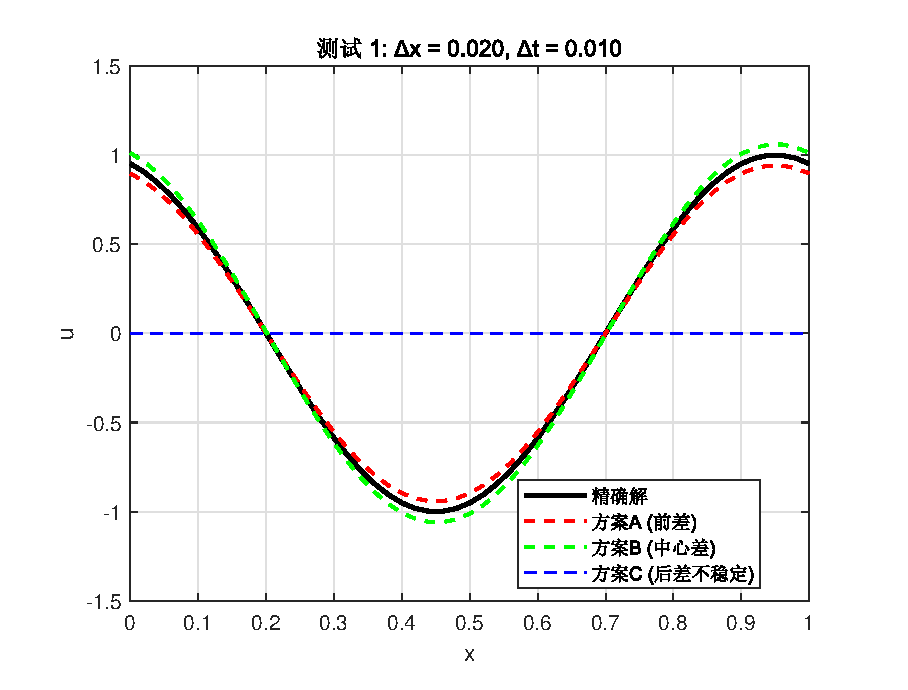
\includegraphics[width=0.8\textwidth]{fig/result_001.eps}
\caption{$\Delta x = 0.02$, $\Delta t = 0.01$ 时的数值解与精确解比较}
\end{figure}

\begin{figure}[H]
\centering
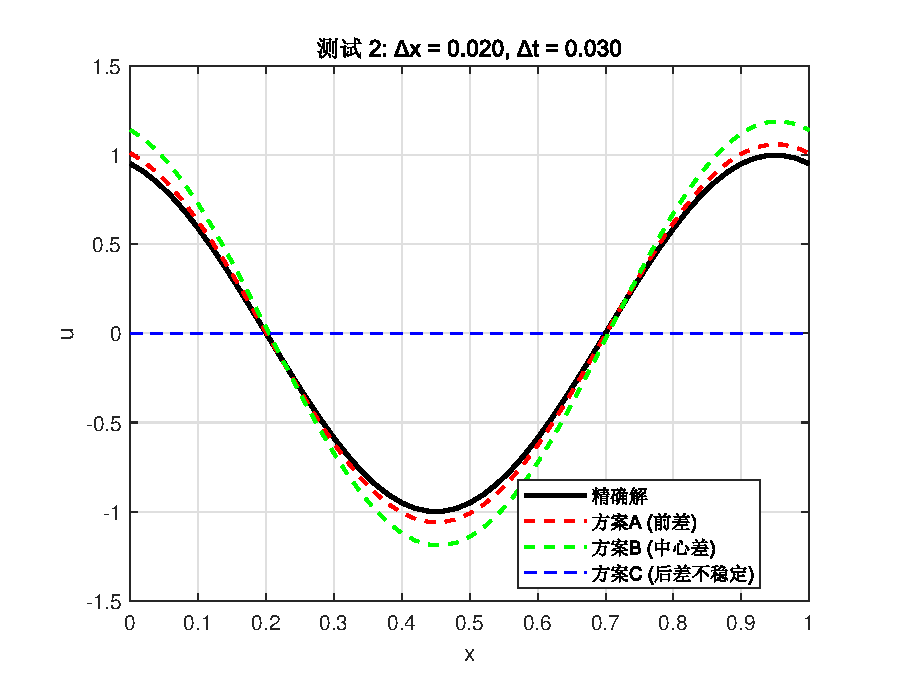
\includegraphics[width=0.8\textwidth]{fig/result_003.eps}
\caption{$\Delta x = 0.02$, $\Delta t = 0.03$ 时的数值解与精确解比较}
\end{figure}

从结果可以看出, 方案 C 在两种情况下都出现了严重的数值不稳定, 误差达到 $10^3$-$10^7$ 量级, 这与理论预测的后差格式无条件不稳定相符. 

然而, 方案 A 和 B 的结果与理论预期存在差异: 当 CFL 数大于 1 时 (测试 2), 理论上方案 A 应该不稳定, 方案 B 应该表现出更强的不稳定性, 但实际误差相对较小. 这可能是因为计算时间较短 ($T_{end} = 0.3$), 不稳定性没有充分发展, 或者是光滑初值延缓了不稳定性的显现.

\subsection{减小步长测试}

为了进一步验证数值方法的稳定性, 我们减小空间和时间的步长, 采用 $\Delta x = 0.002$, 分别测试 $\Delta t = 0.001$ 和 $\Delta t = 0.003$ 的情况.

\begin{table}[H]
\centering
\caption{减小步长测试结果 ($\Delta x = 0.002$)}
\begin{tabular}{cccccc}
\toprule
测试案例 & 方案 & $\Delta t$ & CFL 数 & L2 误差 & 最大误差 \\
\midrule
测试 1 & A & 0.001 & 0.5 & \num{4.178342e-03} & \num{5.904302e-03} \\
       & B & 0.001 & 0.5 & \num{1.130479e-02} & \num{3.612149e-02} \\
       & C & 0.001 & 0.5 & \num{1.110162e+86} & \num{6.815202e+86} \\
\midrule
测试 2 & A & 0.003 & 1.5 & \num{2.399847e+13} & \num{7.477785e+13} \\
       & B & 0.003 & 1.5 & \num{1.041390e+09} & \num{3.857626e+09} \\
       & C & 0.003 & 1.5 & \num{1.091222e+56} & \num{8.341998e+56} \\
\bottomrule
\end{tabular}
\end{table}

\begin{figure}[H]
\centering
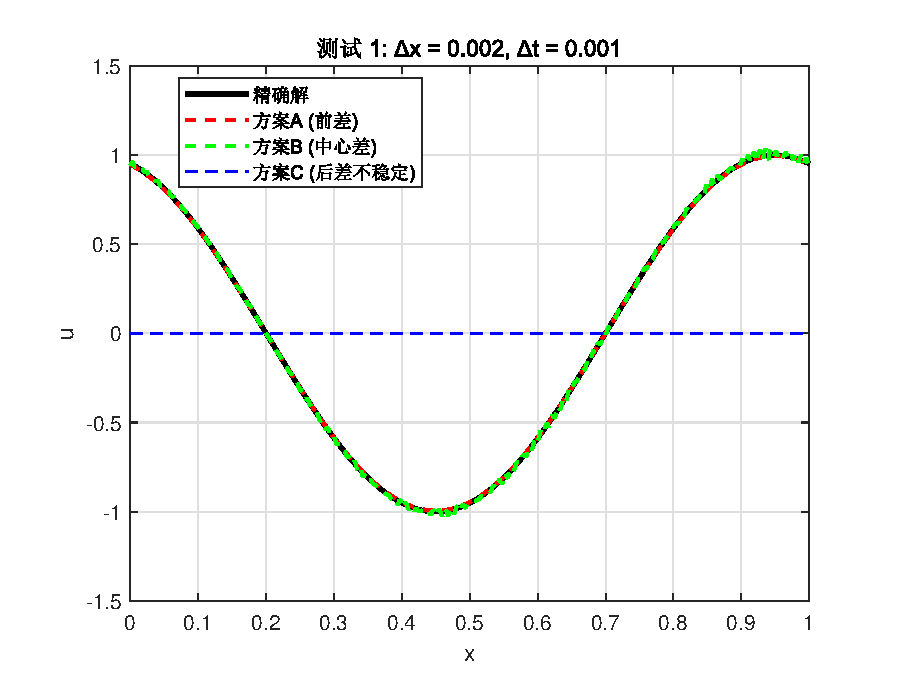
\includegraphics[width=0.8\textwidth]{fig/result_0001.eps}
\caption{$\Delta x = 0.002$, $\Delta t = 0.001$ 时的数值解与精确解比较}
\end{figure}

\begin{figure}[H]
\centering
\includegraphics[width=0.8\textwidth]{fig/result_0003.eps}
\caption{$\Delta x = 0.002$, $\Delta t = 0.003$ 时的数值解与精确解比较}
\end{figure}

在减小步长的测试中, 数值不稳定性更加明显地表现出来:

1. 当 CFL 数等于 0.5 时, 方案 A 和 B 的误差较小, 但方案 C 仍然完全发散.

2. 当 CFL 数等于 1.5 时, 所有三种方案都出现了严重的数值不稳定, 误差达到 $10^9$-$10^{86}$ 量级.

3. 方案 A 在 CFL 数大于 1 时确实表现出不稳定性, 验证了其 CFL 稳定性条件.

4. 方案 B 和 C 在两种 CFL 数下都不稳定, 验证了它们对于纯对流方程的无条件不稳定性.

\section{结论}

通过本实验, 我们得到以下主要结论:

1. 对于方程 $u_t = u_x$, 前差格式 (方案 A) 在 CFL 条件 $\Delta t / \Delta x \leq 1$ 满足时是稳定的, 否则会出现数值不稳定.

2. 中心差格式 (方案 B) 和后差格式 (方案 C) 对于纯对流方程都是无条件不稳定的, 这与理论分析一致.

3. 在初始参数测试中, 由于计算时间较短和初值光滑, 不稳定性没有充分发展, 导致方案 A 和 B 在 CFL 数大于 1 时的误差相对较小.

4. 通过减小步长的进一步测试, 所有格式的稳定性特性都得到了更清晰的验证.

5. 数值实验的结果基本符合理论预测, 验证了不同差分格式的稳定性特性.

本实验强调了在选择数值方法时考虑稳定性条件的重要性, 以及通过数值实验验证理论分析的必要性.

\end{document}
